\section{Process' Perspective}
% SECTION PURPOSE: In essence it has to be clear how code or other artifacts come from idea into the running system and everything that happens on the way.

\subsection{Developer interaction}
In order to handle interactions in an effecient manner, the team met at every lecture and exercise session, where a plan was discussed on how to reach the goal of the following weeks exercises. This plan was then carried out between the developers. In order to work asynchronously, we also decided on using Discord as an online communication tool. The reason this was chosen, was due to the ease of creating a group chanel, where all members could write their topics and update, whilst also being able to join voice calls and share individuals screens. 
\\
Another choice we could have made was to use Microsoft Teams, as this is also how the course provides news and discussions. We opted not to use teams, as all members were more comfortable with Discord and had accounts.

\subsection{Organization of team}\label{subsec:organization_of_team}
The team handled both Agile processes, DevOps practices, Frontend and backend development, therefore a suitable name for the team would be a "Full-Stack DevOps Team". The team was not build by generalists, but rather specialists in the frontend and backend departments. As DevOps is the main intended learning outcome of the course, all team members were responsible for this practice.
\begin{itemize}
    \item \textbf{Agile:} As the course required new implementations and requirements every week, the team is organized in an agile manner, always ready to adapt and respond to changes.
    \item \textbf{DevOps:} Other than migrating the old "minitwit" application into a modern framework, most of the work thereafter was done in devops practices, including monitoring, CI/CD pipelines and more. All developers were responsible for working and implementing the changing feature requirements, provided by the course.
    \item \textbf{Frontend:} 1 of the team members was assigned to the frontend, redesigning the entire application to use a modern frontend framework (Next.js), a long with updating dependencies and improving the UI and UX of the application.
    \item \textbf{Backend:} 3 of the team members worked on the backend, migrating the application from a Python flask API into a Go:GIN application.
\end{itemize}

\subsection{Full stage \& tool description of CI/CD Chains}


\subsubsection{Continuous integration}\label{subsubsec:ci}
We built a continuous integration(CI) workflow\cite{DevOps-CI-CDont} that would serve as a quality gate when pushing new changes. The aim was to define a set of tests that if ever failed we would not want to publish those changes to production. As the main focus of Minitwit was to handle requests from the simulator our tests only related to the backend and no end-to-end tests exist.\\\\
When a push or pull-request is accepted into the main branch, a virtual machine (VM) is spun up containing environment variables needed for establishing a connection to the database, these secrets are fed through GitHub's built-in "github secrets"\cite{GitHub-Secrets}. Once the machine is ready it builds a test-specific Dockerfile that mimics our real Dockerfile but instead connects to a test database rather than production. We then also install DigitalOcean's command line tool "Doctl"\cite{DigitalOcean-doctl}, and push our new image to the Digital Oceans Container registry.\\\\
With this job completed we now have our API running on our virtual machine and we can start testing. Testing happens in a new job so again we spin up a virtual machine that installs doctl but this time it instead pulls the image the other job uploaded and then runs the image before making a call to "go test" running all go tests defined in the repository. Finally, we also have a static code analysis job running that installs all dependencies before running a typescript type check "tsc", eslint, and go vet. If any of these steps fails the job fails and the workflow as a whole exists with a "Failure". 
\subsubsection{Continuous deployment}
To support frequent delivery of new versions of mini twist we also created a continuous deployment(CD) workflow on Github actions. The workflow runs any time the CI workflow completes and the conclusion is "Success", meaning that all jobs succeeded without fail. The workflow then starts a VM that builds the backend and frontend images (along with the necessary secrets stored in github secrets), before installing doctl and pushing the images to the container registry.\\\\
But just pushing them to the registry is not enough as we need to communicate to our digital ocean droplet that a change was made to one of the images. To achieve this we utilize "Watchtower"\cite{watchtower}. Watchtower monitors running docker containers and watches for any changes made to the images that initially started those containers, if any images are updated watchtower will restart the container using the new image. Watchtower is set up on our project to look for a change on any of our images every 60 seconds. The combination of the CD and watchtower means that any time we push code(that passes the quality gate defined in CI) to the main branch it also updates our hosted production server. 

\subsection{Organization of repository}
% describe the structure of of mono-repository 
We decided to structure the repository as a monorepo. We had 2 projects in the repo concerning a frontend project in Next.js and a backend project in Go. The reason we decided for this structure, is that a monorepo allows us to sync releases from one main repository. Meaning every time there is a release, then all of the code is at the same state. Furthermore a monorepo is useful when the codebase is not too large, meaning we do not have thousands of files and or packages in the codebase, slowing down each pull, commit and push.
\\\\
When building micro services a polyrepo can seem to be the natural choice, however what the monorepo allowed us to do was creating a unified and automated build and deploy pipeline, that can mitigate many issues associated with polyrepos, such as not being at the same state \cite{monorepo_pros}. 

\subsection{Applied branching strategy}\label{subsec:branching_strategy}
At the project kick-off we did not have a branching strategy, meaning all development was done on a "Dev" branch, that all developers were working on. This did not cause a lot of issues, as all commits and pushes were short in terms on modified lines of code, leading to no merge conflicts.
\\\\
Later in the project, we developed a dedicated branching strategy, following the GitHub Flow strategy \cite{branching_strategy}. This strategy is dedicated to small teams, having a main, develop, feature and hotfix branch. All developers branch directly from the main branch, such that the main branch which remains stable. All branches are then isolated to work on and can then be merged into main again. The reason we chose this over the GitFlow strategy, is that the GitHub Flow strategy does the same but without release branches. We chose to have all of our releases directly from the main branch, when all work was done. This kept the main branch in a constant deployable state, supporting our CI and CD processes.

\subsection{Applied development process}
We used Github's built-in issue tracking system, eventually also using those issues inside a Kanban-like board via a Github "Project" for the Github organization we had. At the end, we had 4 columns in the board (Todo, In Progress, Done and Unprioritized). Unprioritized recommended all the tasks that we found would be realistic tasks for the project if it were to continue, that weren't prioritized for the course. 
\subsection{Monitoring}
% How do you monitor your systems and what precisely do you monitor?
For our monitoring setup we utilize Prometheus \& Grafana. A Prometheus container scrapes our backend api for metrics on a fixed time interval, and the metrics are visualized by grafana which queries Prometheus. In Grafana we have a single main dashboard with two graphs, specifically graphs for memory usage (\%) and endpoint counter, which can be seen on \autoref{fig:grafana}.
\\\\
For the endpoint counter we gather the metrics using middleware, that gets executed after every request. As we are using the gin framework in Go, we are able to register it like so:
\begin{verbatim}
...
Router.GET("/metrics", gin.WrapH(promHandler))
Router.GET("/mytimeline", getTimeline, incrementCounter(m, "/mytimeline"))
Router.GET("/public", getPublicTimeline, incrementCounter(m, "/public"))
...
\end{verbatim}
The \textit{incrementCounter} function is just a helper function we created, which returns a "gin.Handlerfunc", which will count the appropiate endpoint once triggered e.g. "/mytimeline".
\\\\
For recording the memory usage, we simply have a goroutine in the background which records the current memory usage every 10 seconds. Promtheus will scrape our api this information from the "/metrics" endpoint at a fixed interval.
\\\\

\begin{figure}[H]
    \centering
    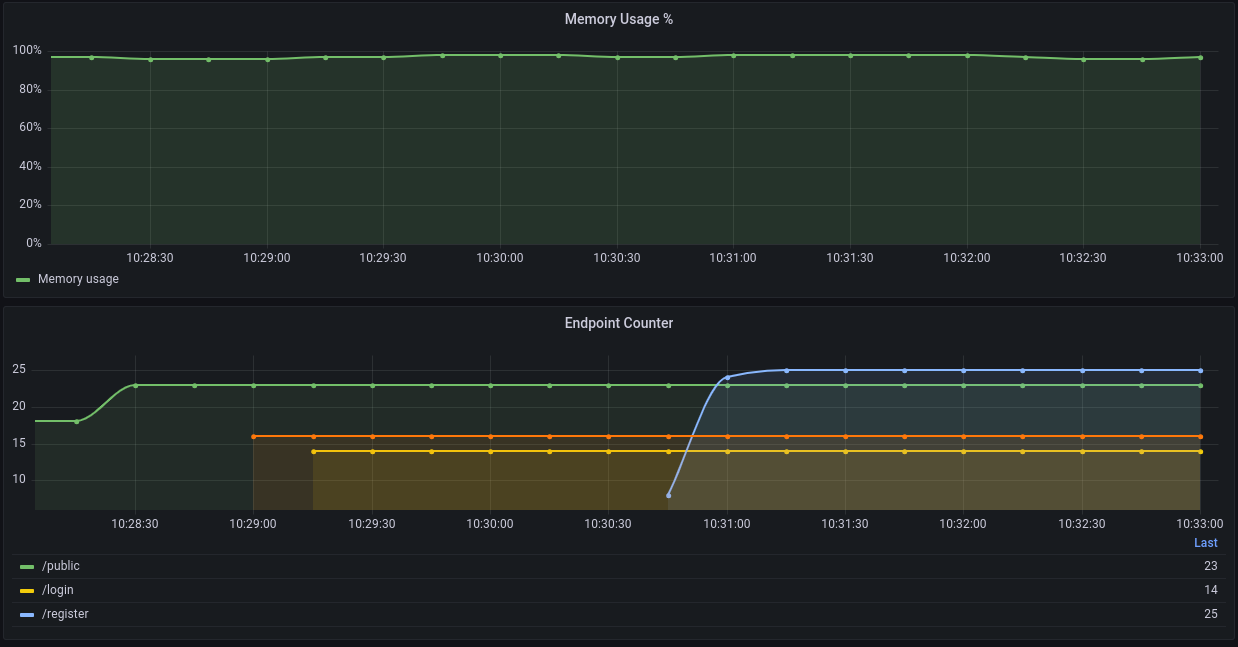
\includegraphics[scale=0.35]{report/diagrams/grafana_example.png}
    \caption{The grafana dashboard after executing some requests to the /public, /login, and /register endpoints.}
    \label{fig:grafana}
\end{figure}
%DigitalOcean resource alerts and uptime (\url{http://cicdont.live/public})
\subsection{Logging}
% What do you log in your systems and how do you aggregate logs?
Our logging system consists of an EFK stack, i.e. elasticsearch, filebeat and kibana. Filebeat captures and ships the logs from standard out to  elasticsearch, and kibana is the user interface that allows us to retrieve the logs. As we did not implement docker swarm/load balancing, there was log aggregation from different sources. \\
We abandoned plans of implementing Docker Swarm, due to time constraints. As such, we have no automatic load balancing or scaling strategy. We can however with a 
\subsection{Security assessment}
% Brief results
The exercises for lecture 9 was to do a security assessment of the minitwit application. Our peer group sadly did not leave an assesment of our website, which is why we did it ourselves. For this, we used Skipfish \cite{skipfish}. Skipfish is a security reconnaissance tool, that gives an output of potential security risks. Running this tool on our website does not bring return any interesting security risks\footnote{Skipfish results: \url{https://github.com/DevOps-CI-CDont/DevOps-CI-CDont/tree/main/CICdont3.html}}.
\\\\
To answer some of the questions for the security assesment on lecture 9, we can give a reasoning to the security of our website:
\begin{enumerate}
    \item \textbf{HTTPS}: The website does not support HTTPS. For a short moment, we had a SSL certificate set up through Cloudflare, such that all traffic was considered safe. This caused an issue for all the API calls, which were hosted on a port that was not on HTTPS, but rather HTTP. HTTPS states that you cannot make calls to non-secure HTTP sites, meaning that all our API calls failed. Due to time restrictions, we were unable to fix this issue, which is why the website is still hosted on HTTP.
    \item \textbf{SQL injection attacks (XSS)}: The frontend handles user logins and signup and more through input fields, which are sent directly to the backend API. In the backend, strings are never executed directly against the database, instead, an ORM interface sits between the user and the database, this makes it impossible for the user to inject SQL. 
    \item \textbf{Frontend packages}: When dealing with external packages and dependencies, we may be subject to a zero day exploit. If there is discovered a XSS, prototype pollution or other kinds of attacks in a package, then we are left behind and stuck until a fix is created. For npm packages, we can run an audit, to check state of direct and indirect dependencies. Running an audit as of the handin date, there are no security risks with external packages.
    \item \textbf{Authentication}: One of the biggests risks in our application is the authentication system. Not the signup or login process, but the way authentication is handled. Currently, when you login in the frontend, the backend sends your user ID back which is then set as a \verb|user_id| cookie. This is not optimal, as any user can login as any other user, by simply changing the \verb|user_id| cookie. A better way of doing this would be to implement JSON Web Tokens (JWT) \cite{jwt}, but again, due to time restrictions this was discarded.
\end{enumerate}

\subsection{Applied strategy for scaling and load balancing}
Before trying to use Docker Swarm, our only scaling had been vertical: increasing resources for CPU, RAM, and Disk on a single Virtual Machine (Droplet). It has also been manual, meaning we have to notice resource usage on the droplet and go into DigitalOcean to upscale resources (during which the Droplet must be turned off). We had configured some resource alerts in DigitalOcean (Memory Usage percent and CPU utilization percent, sending an email if either is above 85\% for 15 minutes or longer). 

\subsection{AI assistants}
% Reflect how it supported/hindered your process.
We have used Github Copilot via its VSCode extension.
A couple of areas where it was memorably useful:
\begin{enumerate}
    \item writing out repetitive patterns in the API (eg. error handling in Go, checking for certain parameters/cookies).
    \item writing fetch requests from the frontend (it seems to understand well how to use the endpoints that are described in the same repository).
    \item writing utility functions (Copilot is especially effective if given a perfectly descriptive function name, even better if standard terminology is used)
\end{enumerate} 
One challenge of using Copilot with an unfamiliar language (such as Go was to all of us), is that it can be really hard to tell if a suggestion is correct. Even if something seems to work as intended, it is still important to understand the code. \\\\
Another "AI Assistant" we have used is ChatGPT. A couple of areas where it was memorably useful: 
\begin{enumerate}
    \item Suggesting and explaining nginx configurations
    \item Debugging CORS errors, suggesting fixes with middleware in Go backend.
    \item Debugging memory usage problems. 
    \item Generating commands for iptables configuration.
\end{enumerate}
The conversational design is quite nice to be able to "tweak" its suggestions. It often spits out large blocks of code that aren't quite what you want, but it can fix that if told what to tweak. \\
A downside is that it may \textit{hallucinate} commands, flags, and functions that seem very plausible and one may think "How great! That command is exactly what I want", and then it doesn't exist. \\
When asked to use the functionality of a library, it will tend to use it in the way that there is most content like on the internet - this means the newest "best practices" aren't as likely to be used as whatever is still most common in the training data.  